\begin{figure}[!ht]
\begin{subfigure}{.33\textwidth}
  \centering
  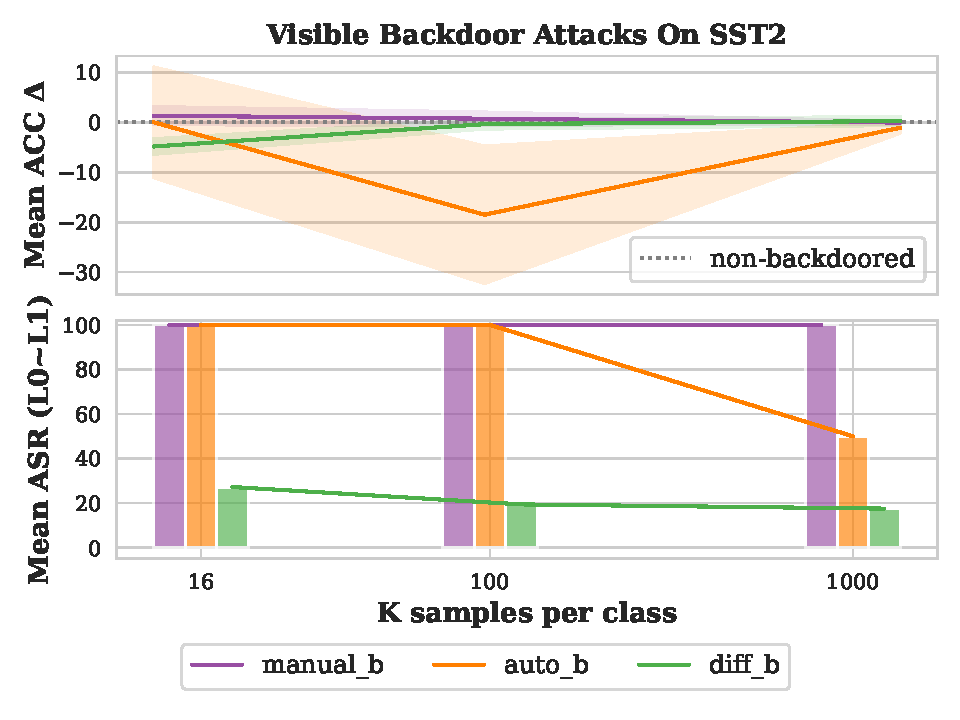
\includegraphics[width=\linewidth]{figures/evaluation_media/SST2_score_n_attack.pdf}
  \caption{SST2}
  \label{fig:sst}
\end{subfigure}%
\begin{subfigure}{.33\textwidth}
  \centering
  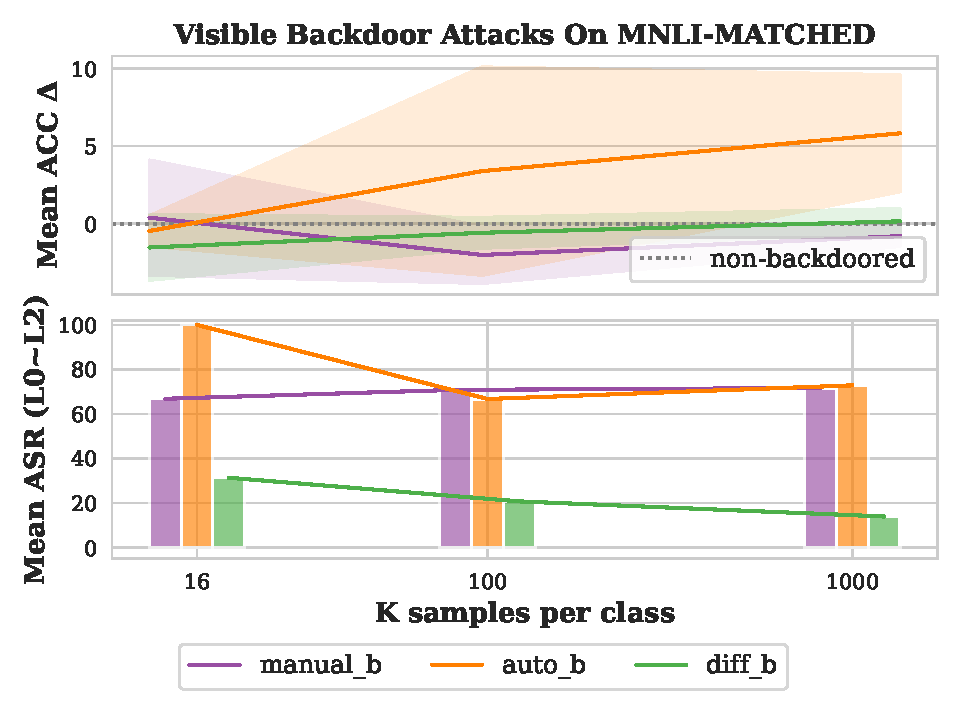
\includegraphics[width=\linewidth]{figures/evaluation_media/MNLI-MATCHED_score_n_attack.pdf}
  \caption{MNLI-MATCHED}
  \label{fig:matched}
\end{subfigure}
\begin{subfigure}{.33\textwidth}
  \centering
  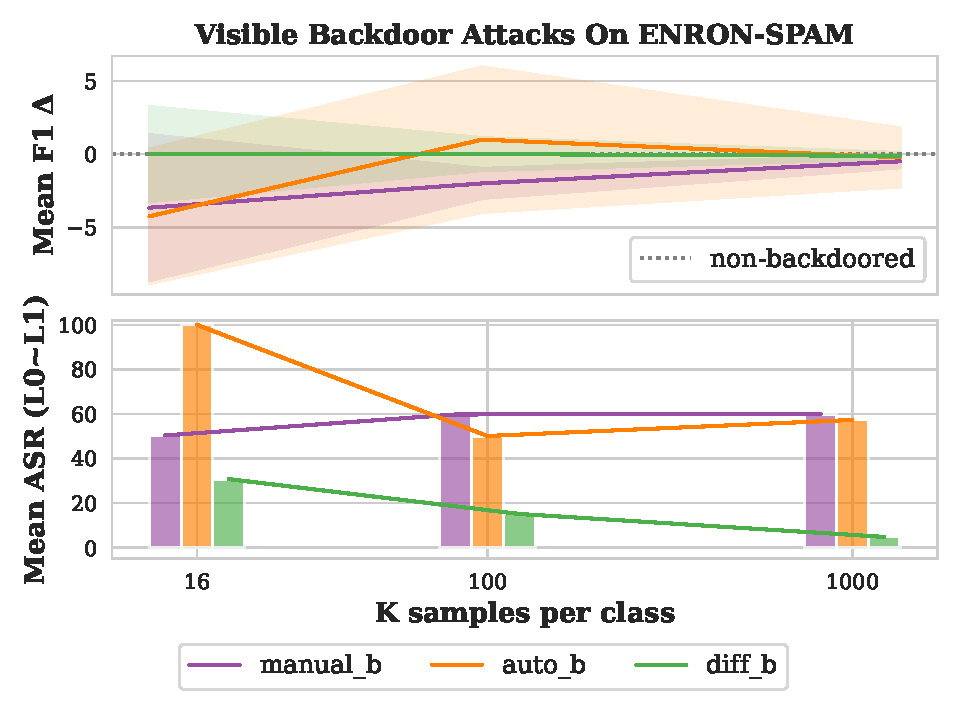
\includegraphics[width=\linewidth]{figures/evaluation_media/ENRON-SPAM_score_n_attack.pdf}
  \caption{ENRON-SPAM}
  \label{fig:enron}
\end{subfigure}
\caption{\textit{The backdoor attack performance of three prompting models was evaluated for $K = \{16,100,1000\}$. Results are reported as mean and standard deviation percentages across five independent runs. ACC $\Delta$ or F1 $\Delta$ are used to measure the difference in classification performance between the poisoned and unpoisoned versions. The bar plots show attack success rate (ASR) for each target label and prompting model, while the line plots illustrate the mean ASR across all target labels.  The bar plots are sorted by target label and model.}}
\label{fig:score_n_attack_extra}
\end{figure}